% TikZ pipeline diagram for the RRPR 2026 paper.
%
% Compile standalone with:
%   pdflatex --output-directory=paper/figures/_build paper/figures/fig1_pipeline.tex
% but it is normally \input directly into main.tex.
\documentclass[border=4pt]{standalone}
\usepackage{tikz}
\usetikzlibrary{positioning,arrows.meta,calc,fit,backgrounds,shadows}

\begin{document}
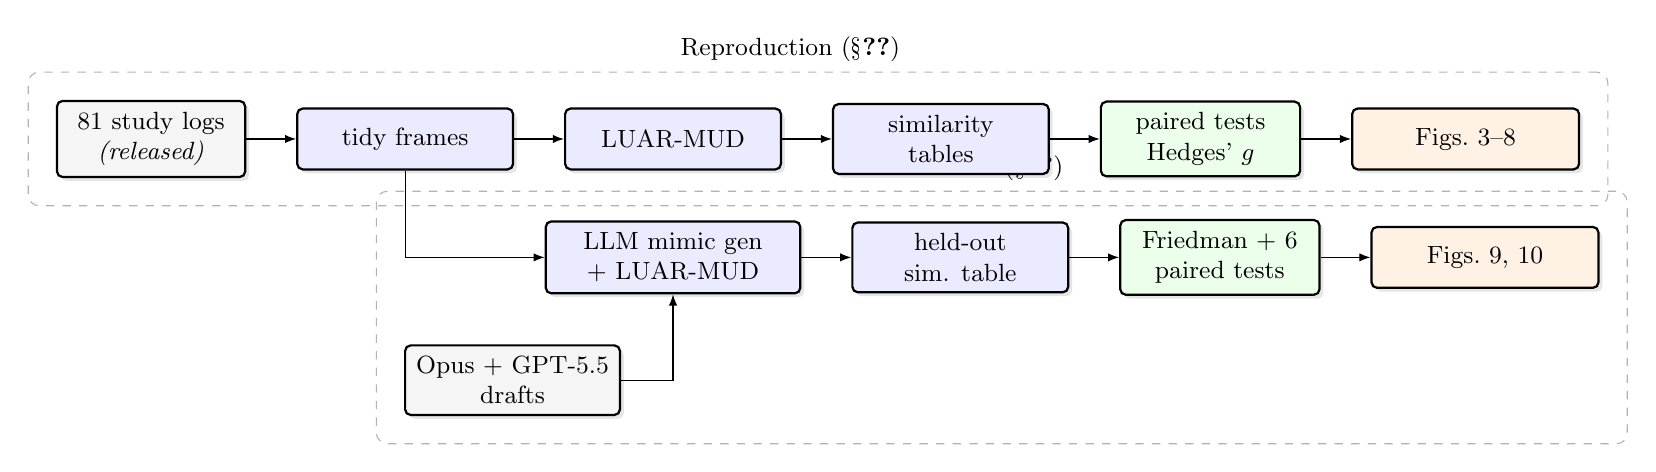
\begin{tikzpicture}[
  font=\small,
  node distance=10pt and 18pt,
  box/.style={
    draw, thick, rounded corners=2pt, minimum height=22pt,
    inner sep=4pt, align=center,
    drop shadow={opacity=0.20, shadow xshift=1.4pt, shadow yshift=-1.4pt}
  },
  data/.style={box, fill=black!4, minimum width=68pt},
  proc/.style={box, fill=blue!8, minimum width=78pt},
  test/.style={box, fill=green!8, minimum width=72pt},
  outbox/.style={box, fill=orange!10, minimum width=82pt},
  >={Latex[length=4pt]}
]
  \node[data] (logs)   {81 study logs\\\textit{(released)}};
  \node[proc, right=of logs]  (tidy)   {tidy frames};
  \node[proc, right=of tidy]  (luar)   {LUAR-MUD};
  \node[proc, right=of luar]  (sim)    {similarity\\tables};
  \node[test, right=of sim]   (tests)  {paired tests\\Hedges' $g$};
  \node[outbox, right=of tests] (figs)  {Figs.~3--8};

  \node[proc, below=18pt of luar, minimum width=92pt]
        (gen) {LLM mimic gen\\+ LUAR-MUD};
  \node[proc, right=of gen] (mimsim) {held-out\\sim. table};
  \node[test, right=of mimsim] (final) {Friedman + 6\\paired tests};
  \node[outbox, right=of final] (fig9)  {Figs.~9, 10};

  \node[data, below=18pt of gen, xshift=-58pt] (drafts) {Opus + GPT-5.5\\drafts};

  \draw[->] (logs)  -- (tidy);
  \draw[->] (tidy)  -- (luar);
  \draw[->] (luar)  -- (sim);
  \draw[->] (sim)   -- (tests);
  \draw[->] (tests) -- (figs);

  \draw[->] (tidy.south) |- (gen.west);
  \draw[->] (drafts) -| (gen.south);
  \draw[->] (gen) -- (mimsim);
  \draw[->] (mimsim) -- (final);
  \draw[->] (final) -- (fig9);

  \begin{pgfonlayer}{background}
    \node[draw=black!30, dashed, rounded corners=4pt,
          fit=(logs)(tidy)(luar)(sim)(tests)(figs),
          inner sep=10pt, label={[xshift=-10pt]above:Reproduction (\S\ref{sec:repro-results})}] {};
    \node[draw=black!30, dashed, rounded corners=4pt,
          fit=(drafts)(gen)(mimsim)(final)(fig9),
          inner sep=10pt, label={[xshift=-10pt]above:Extension (\S\ref{sec:extension})}] {};
  \end{pgfonlayer}
\end{tikzpicture}
\end{document}
